\documentclass{article}
\usepackage[utf8]{inputenc}
\usepackage{amsmath}
\usepackage{graphicx}
%\usepackage{url}
\usepackage{hyperref}
\usepackage[strict]{changepage}


\title{It-sikkerhed: A3}
\author{Christian Påbøl og Silja Knudsen }
\date{September 2020}

\begin{document}

\maketitle

\section{Review Questions}
\subsection{7.5}
In this question, we wish to answer why so many DoS attacks use packets with spoofed source addresses.\\

When the attacker uses spoofed source addresses, the the destination host will try to send a response back to the spoofed address and then wait for a second response from this address (3-way handshake). Since this address did not start a connection, it will response with an error message back. Thus, the destination host  uses time and resources on starting a false connection, which could have been used to establish real connections. 
Another thing, the attacker could do, is to set the source address to a non existing address. In this case, the destination host will also try to establish a connection and wait for the source host to reply. But since the source address does not exist, the the destination host will not receive any answer. The destination host will try to establish the connection a couple of times before it determines that the source address will not respond and then ends the connection. Again, the destination host have wasted its time and resources. By sending a lot of messages with a false source address, the attacker is able to use up all of the destination host's resources and thus make it unable to establish connection to any real users.


\subsection{7.7}
In this question, we wish to answer what the difference between a DDoS attack and a classic DoS attack is, and why DDoS attacks are considered more potent than classic DoS attacks.\\

In a DoS attack, the attacker tries to overload a server by flooding the servers resources and thus make it unable to respond to its real users. All of the packages in this attack is send from the same source system. In a DDoS attack, the attacker will also try to overload a server, but instead of using one system, the attacker will use multiple of systems to overload the server. The attacker uses malware to subvert the systems and then install an attack agent, which the attacker will use to control the systems. The attacker can thus send a command to systems telling them to attack the server by overloading its resources. \\ 
Thus, the difference in a DoS and DDoS attack is the scope of the attack. A DDoS attack can be much more massive and harder to track back to the actual attacker, since the flooding comes from a lot of other systems. This is also the reason that DDoS attacks are considered more potent than DoS attacks.

\subsection{9.1}
In this question, we wish to list the difference types of firewalls.\\ 
\begin{itemize}
    \item Packet Filtering Firewall - this firewall uses a filter consisting of some rules, that determine whether the packet is allowed from the information contained in the packet header. The rules can be based on the IP addresses of both the source and the destination as well as the port number. If a packet does not match any of the rules in the filter, a default action must be taken - this will usually be not to allow the packet to pass the firewall. 
    
    \item Stateful Inspection Firewalls - this firewall uses a directory containing those TCP connections, that has been established and allows packets from those connections. It combines this check with some filtering of the packet header. 
    
    \item Application-Level Gateway - this firewall acts as a proxy for the original server. Whenever a client wishes to connect or request something from the server, the client will first connect to the proxy and provide a user ID together with some other authentication information. If this information is valid, the proxy will then allow the client to connect to the original server. 
    
    \item Circuit-Level Gateway - this firewall checks whether a packet is allowed from the connection the packet belongs to. The firewall perform this check by using a table containing all established connections. 
\end{itemize}


\subsection{9.3}
In this question, we wish to answer which types of attack is possible on a packet filtering firewall?\\

\begin{itemize}
    \item IP address spoofing - the attacker will change the IP address of the packet so it matches the IP address of an internal host. If packets from this internal host is allowed through the firewall, the attacker is able to transmit packets to the target system. 
    
    \item Source routing attacks - the attacker will try to find a route across the internet to the target, which will bypass any security measures and thereby, also the firewall. 
    
    \item Tiny fragment attacks - the attacker will create small fragments, in which one of the fragments contains the TCP header information. The attacker then hopes that the firewall only examines the fragment containing the header information by sending this fragment as the first fragment and thus allowing the other fragments to pass the firewall. 
\end{itemize}


\subsection{9.10}
In this question, we wish to answer why it is useful to have host-based firewalls.\\

Host-based firewalls runs on a individual system and thus protect the system from any suspicious incoming or outgoing connections. This means that the security in which what packets are allowed to pass to the systems does not depend on the security of the network and router, that connects the system to the internet. Thus, the system will still be able to protect it self even though it is connected to a network with low security measures. 

\subsection{13.2}
In this question, we wish to list and briefly define the three cloud service models.

\begin{itemize}
    \item Software as a Service - this is software applications, that runs on a cloud server. An example of this is gmail or google docs. 

\item Platform as a Service - this is platform-based services, that allows users to develop and manage applications. An example of this is an database hosted on a cloud server. 

\item Infrastructure as a Service - this is services that provides computing resources hosted on a cloud server. An example of this is virtual machines. 
\end{itemize}

\subsection{13.4}
In this question we describe some of the main cloud-specific security threats. \\
The Cload Security Alliance lists the following as the top cloud specific security
threats:
\begin{itemize}
    \item \textbf{Abuse and nefarious use of cloud computing} - When renting servers
    out you give a possibly nefarious actor access to your internal cloud. You also
    risk spammers using your site to send out malware and scam emails.\\
    \item \textbf{Insecure Interfaces and APIs} - Most CSPs provide APIs to control
    and deploy services and servers. If these basic apis fail, you can end up with
    a malicious actor spinning up servers left and right under someone elses billing
    account.\\
    \item \textbf{Malicious Insiders} - When using a CSP an organization gives up a
    tremendous amount of control and insight, opening themselves up to a sort of
    cyber supply chain attack. If an insider at the CSP(or an actor having gained
    control) wants to steal data, they can do so without ever touching the organizations
    front-end code\\
    \item \textbf{Shared technology issues} - Most of the services offered by cloud
    providers exist on shared hardware, which generally isn't built to be secure
    in a multi-tenant system. While providers spin up virtual machines for the
    individual tenants, they open themselves up to side-channel attacks and the
    much scarier sandbox escapes. If an attacker gains access to a vm host, all
    underlying services could be breached.\\
    \item \textbf{Data loss or leakage} - Is pretty self-explanatory and a general
    issue in deployment of web applications or databases.\\
    \item \textbf{Account or service hijacking} - If an intelligent adversary gains
    access to an account or set of credentials, an organization can experience a breach
    of confidentiality, integrity and availabillity.\\
\end{itemize}


\section{Problems}

\subsection{7.4}
In this exercise, we wish to answer the following problems: \\

\textit{In order to implement a DNS amplification attack, the attacker must trigger the creation of a sufficiently large volume of DNS response packets from the intermediary to exceed the capacity of the link to the target organization. Consider an attack where the DNS response packets are 100 bytes in size (ignoring framing overhead). How many of these packets per second must the attacker trigger to flood a target organization using an 8-Mbps link? If packet size is 1000 bytes? Or 1500 bytes? If the DNS request packet to the intermediary is 70 bytes in size, how much bandwidth does the attacker consume out of the 8-Mbps link to send the necessary rate of DNS request packets?}\\
 

Using a DNS response packet with size of 100 bytes, it would take 
$\frac{8 \text{ Mbps}}{100 \text{ bytes}} = \frac{1,000,000 \text{ bytes per second}}{100 \text{ bytes}} = 1000 \text{ packets per second}$
to flood the organization. \\ 

Using a DNS response packet with size of 1000 bytes, it would take 
$\frac{8 \text{ Mbps}}{1000 \text{ bytes}} = \frac{1,000,000 \text{ bytes per second}}{1000 \text{ bytes}} = 1,00 \text{ packets per second}$ 
to flood the organization. \\

Using a DNS response packet with size of 1500 bytes, it would take 
$\frac{8 \text{ Mbps}}{1500 \text{ bytes}} = \frac{1,000,000 \text{ bytes per second}}{1500 \text{ bytes}} = 66.667 \text{ packets per second}$ 
to flood the organization. \\
 
The amount of bandwidth, the attacker will consume depends on the size of the response packet. For each above response packet sizes, the amount of bandwidth will be \\

1,000 packets per second * 70 bytes per intermediary DNS request packet = 70,000 bytes per second\\

100 packets per second * 70 bytes per intermediary DNS request packet = 7,000 bytes per second\\

66.667 packets per second * 70 bytes per intermediary DNS request packet = 4,666.69 bytes per second



\subsection{9.11}
I set up the following packet-filtering table for the firewall:\\
\begin{table}[!htb]
    \begin{adjustwidth}{-1.8in}{-1in}
    \centering
    \small
\begin{tabular}{|c|c|c|c|c|c|c|c|}
Rule & Direction & Src adress & Dst adress & Protocol & Dst port & Action & Comment\\\hline
1 & In & External & DMZ & TCP & 25,465,587 & Allow & External to relay\\
2 & In & Internal & DMZ & TCP & 25,465,587 & Allow & External to relay\\
3 & In & External & Internal & TCP & 25,465,587 & Reject & External directly to Internal\\
4 & In & Internal & External & TCP & 25,465,587 & Reject & Internal directly to External\\
5 & In & Internal & DMZ MAIL GATEWAY & TCP & 110,995 & Allow & Let insiders access their mail\\
6 & In & External & DMZ MAIL GATEWAY & TCP & 995 & Allow & Let outsiders access their mail only on pop3s\\
7 & In & External & DMZ MAIL GATEWAY & TCP & 110 & Deny & Let outsiders access their mail only on pop3s\\
8 & Out & Internal & External & TCP & 80 & Reject & Force users to use web proxy \\
9 & Out & DMZ & External & TCP & 80 & Allow & Force users to use web proxy \\
10 & In & External & DMZ & TCP & 80 & Allow & Allow anyone to make web requests to web server\\
11 & In & Internal & DMZ & Any & 53 & Allow & Allow Insiders to make DNS requests\\
12 & In & External & DMZ & Any & 53 & Allow & Allow outsiders to make DNS requests\\
13 & In & Internal(Trusted) & DMZ & TCP & 22 & Allow & DMZ Management\\
14 & In & Internal(Trusted) & FIREWALL & TCP & 161 & Allow & Firewall Management\\
14 & Out & FIREWALL & Internal(Trusted) & TCP & 162 & Allow & Firewall Management\\
15 & Any & Any & Any & Any & Any & Reject & Deny all other traffic\\
\end{tabular}
    \caption{Caption}
    \label{tab:my_label}
    \end{adjustwidth}
\end{table}

\newpage
\section{SEED Labs}
In this week lab session, we're working with firewalls, using the iptables userland
configuration tool. Networking on linux is baked into the kernel as a set of tables,
chains and targets. Each table contains a set of chains, and chains contain a set
of rules, which each incoming or outgoing packet runs through. Outside of the set
rules, each chain has a policy target, which determines the default action. We
manipulate these using the commandline tool \verb!iptables!.\\
% Include flowchart
%% notes task 1
\subsection{Task 1: Basic IPTables usage}
To start off with, we have to get a bit familiar with iptables and how to use it. We
start off wanting to block telnet connections which lie on port 23. To do that we
use the command:\\
\verb!iptables -A INPUT -p tcp --dport 23 -j REJECT!\\
To break it down: \verb!-A INPUT! tells us we are appending to the "INPUT" Chain.
\verb!-p tcp --dport 23! is the firewall rule. We want to target the protocol tcp,
with a destination port 23. Finally \verb!-j REJECT! is the jump target. There are
three commonly used jump targets: "ACCEPT", "REJECT" and user-defined chains. ACCEPT
and REJECT are pretty self-explanatory and User-defined chains are used to create
more sophisticated rulesets. One could imagine a user-defined chain that every
packet on port 23 gets sent to, which checks against a list of accepted source ips
and performs other sanity checks. An admin can then just add a single rule to the
INPUT/OUTPUT chains to enable/disable telnet filtering.\\
Below i show terminal output after blocking input and output telnet connections,
with a "main" vm with a firewall and a "clone" vm which acts as a target.
% IPTables after blocking input telnet connections
\begin{verbatim}
root@VM:/home/seed# iptables -A INPUT -p tcp --dport 23 -j REJECT
root@VM:/home/seed# iptables -nvL
Chain INPUT (policy ACCEPT 51 packets, 3524 bytes)
 pkts bytes target     prot opt in     out     source               destination
    0     0 REJECT     tcp  --  *      *       0.0.0.0/0            0.0.0.0/0            tcp dpt:23 reject-with icmp-port-unreachable

[Clone]: root@VM:/home/seed# telnet <main_ip> 
[Clone]: telnet: Unable to connect to remote host: Connection refused
... 
root@VM:/home/seed# iptables -A OUTPUT -p tcp --dport 23 -j REJECT
root@VM:/home/seed# iptables -nvL
Chain INPUT (policy ACCEPT 9 packets, 636 bytes)
 pkts bytes target     prot opt in     out     source               destination
    1    60 REJECT     tcp  --  *      *       0.0.0.0/0            0.0.0.0/0            tcp dpt:23 reject-with icmp-port-unreachable

Chain OUTPUT (policy ACCEPT 5 packets, 664 bytes)
 pkts bytes target     prot opt in     out     source               destination
    0     0 REJECT     tcp  --  *      *       0.0.0.0/0            0.0.0.0/0            tcp dpt:23 reject-with icmp-port-unreachable
root@VM:/home/seed# telnet <Clone_IP>
Trying <CLONE_IP>...
telnet: Unable to connect to remote host: Connection refused
\end{verbatim}
And as seen, our INPUT/OUTPUT rules get added, and telnet connections get blocked
accordingly.\\

For a more interesting challenge, we want to block access to an external website.
I have chosen my own website "cshare.dk" to perform the next tasks, since i control
it, and know it has a static ip.\\
To block outgoing traffic to this site, i find the ip from the domain name, using
the "dig" command. Then i add the following rule:\\
\verb!-p tcp -d 138.68.162.5 --match multiport --dport 80,443 -j REJECT!. Two new
parameters come into play: -d for the destination, in this case the websites IP, and
-match multiport, which tells iptables to filter on more than one port. In this case
i want to block both port 80 for http traffic and port 443 for https traffic. Below
is a slightly edited terminal session:
% Connecting to cshare.dk
\begin{verbatim}
root@VM:/home/seed# dig -t A cshare.dk
; <<>> DiG 9.10.3-P4-Ubuntu <<>> -t A cshare.dk
;; ANSWER SECTION:
cshare.dk.              3580    IN      A       138.68.162.5
root@VM:/home/seed# iptables -A OUTPUT -p tcp -d 138.68.162.5 --match multiport --dport 80,443 -j REJECT
root@VM:/home/seed# iptables -nvL --line-numbers
Chain OUTPUT (policy ACCEPT 6 packets, 808 bytes)
num   pkts bytes target     prot opt in     out     source               destination
1        2   120 REJECT     tcp  --  *      *       0.0.0.0/0            0.0.0.0/0            tcp dpt:23 reject-with icmp-port-unreachable
2        0     0 REJECT     tcp  --  *      *       0.0.0.0/0            138.68.162.5         multiport dports 80,443 reject-with icmp-port-unreachable
root@VM:/home/seed# curl cshare.dk
curl: (7) Failed to connect to cshare.dk port 80: Connection refused
root@VM:/home/seed# curl "https://cshare.dk"
curl: (7) Failed to connect to cshare.dk port 443: Connection refused
root@VM:/home/seed# ssh cshare.dk
root@cshare.dk's password:
\end{verbatim}
As can be seen, after these firewall rules i can still use "ssh" to access the server,
but both http and https traffic results in a "Connection refused".\\


\subsection{Task 3: Getting around our simple firewall}
Now that we have set up a basic firewall, filtering Telnet packets and access to
a website, we want to see how to bypass this, using ssh to create a tunnel. 
Tunnels are described by the arch wiki as "using a protocol of higher level 
to transport a lower level protocol"\footnote{See \url{https://wiki.archlinux.org/index.php/HTTP_tunneling}}
SSH tunnels are a useful way to tunnel traffic through an encrypted connection, and
are used outside of it-security for a variety of purposes. In it-security we see
it being used to bypass firewalls as today. They are also used to create a 
gateway to access more secure services on internal networks.\\

We set up an ssh tunnel to our "clone" vm, and show how, even though telnet 
connections are blocked, we can still use the tunnel on port 8000 to get through.
% Task 3.a
\begin{verbatim}
[09/26/20]root@VM:/home/seed# ssh -L 8000:192.168.122.43:23  seed@192.168.122.43
[09/26/20]seed@VM:~$ telnet 192.168.122.43
Trying 192.168.122.43...
telnet: Unable to connect to remote host: Connection refused
[09/26/20]seed@VM:~$ telnet localhost 8000
Trying 127.0.0.1...
Connected to localhost.
Ubuntu 16.04.2 LTS
VM login: seed
Password:
Last login: Sat Sep 26 12:19:46 EDT 2020 from 192.168.122.43 on pts/19
Welcome to Ubuntu 16.04.2 LTS (GNU/Linux 4.8.0-36-generic i686)
[09/26/20]seed@VM:~$ ip addr
2: ens3: <BROADCAST,MULTICAST,UP,LOWER_UP> mtu 1500 qdisc pfifo_fast state UP group default qlen 1000
    link/ether 52:54:00:d1:a3:28 brd ff:ff:ff:ff:ff:ff
    inet 192.168.122.43/24 brd 192.168.122.255 scope global dynamic ens3
       valid_lft 3590sec preferred_lft 3590sec
    inet6 fe80::a3c5:be50:5aae:912f/64 scope link
       valid_lft forever preferred_lft forever
[09/26/20]seed@VM:~$
\end{verbatim}

SSH tunnels are more powerful than just filtering one port however, and we now set up
a more sophisticated tunnel, using the command \verb!ssh -D 9000 -C seed@192.168.122.43!.
This can be used as a SOCKS proxy in firefox to access the blocked site. On figure
\ref{fig:blockedsite} we see firefox failing to load the webpage before setting the
proxy up, and successfully connecting afterwards.\\
\begin{figure}[!htb]
    \centering
    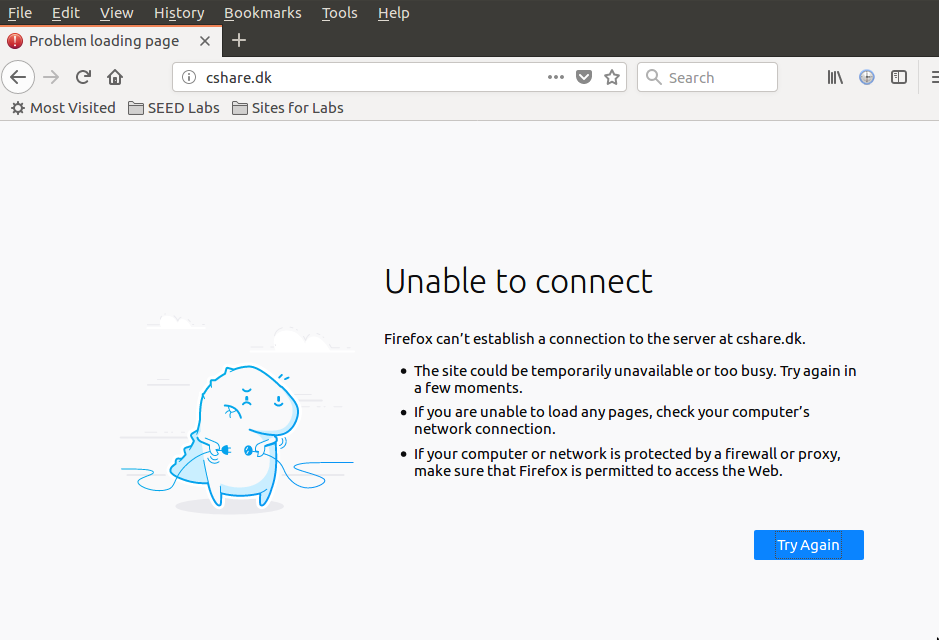
\includegraphics[width=0.95\linewidth]{capture1.png}
    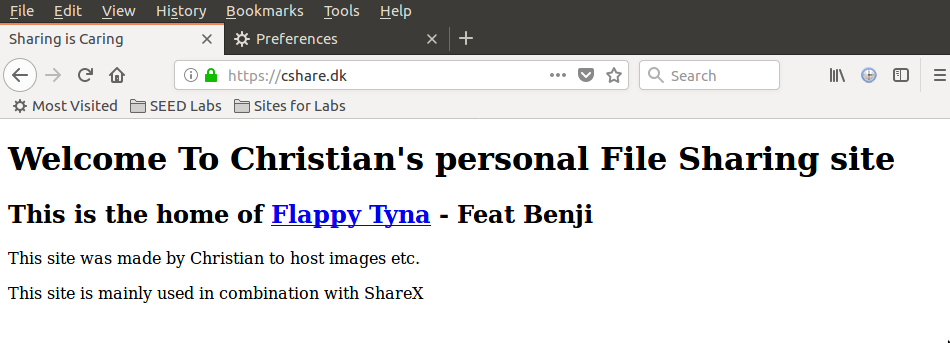
\includegraphics[width=0.95\linewidth]{capture2.png}
    \caption{Firefox showing the website being blocked by our iptables firewall(Top)
    and being able to successfully connect after setting up our proxy(Bottom)}
    \label{fig:blockedsite}
\end{figure}

We inspect the traffic in wireshark afterwards. On figure \ref{fig:wireshark} we see
a dns response on the A and AAAA names, responding with the requested ip. Later
on in the capture, i captured a tls handshake. We see the source and destination ips
being localhost, but the actual packets show we're connecting to a https website with
a lets encrypt certificate. This matches what i'm expecting, since that is what i use
to encrypt traffic to my website. This handshake can be seen on figure 
\ref{fig:wireshark2}.
\begin{figure}
    \centering
    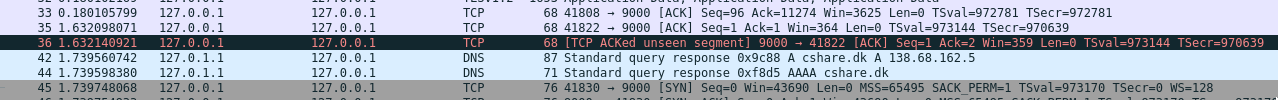
\includegraphics[width=0.7\linewidth]{dns_exchange.png}
    \caption{A dns request being made and fulfilled on localhost}
    \label{fig:wireshark}
\end{figure}
\begin{figure}
    \centering
    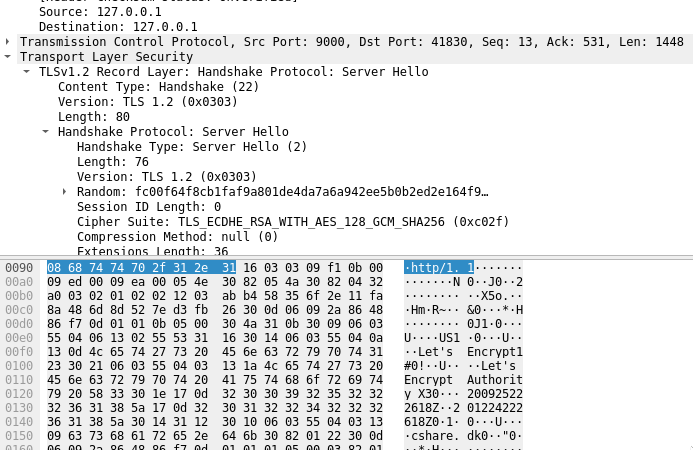
\includegraphics[width=0.7\linewidth]{tls_handshake_with_le.png}
    \caption{A TLS handshake with the lets encrypt certificate header visible}
    \label{fig:wireshark2}
\end{figure}
\subsection{Conclusion}
During this lab we got a cursory introduction to the kernel filtering tables, and the
tool iptables. We set up some rules blocking different types of traffic. After that
we learned how to use tunnels, in this case ssh, to bypass the previously defined rules.
All of this is useful, both to protect and defend against attackers(and unproductive
workers), and to perform red team testing, extracting information and making encrypted
connections outside a firewall.
\end{document}
